\documentclass[conference,a4paper]{IEEEtran}

\usepackage{cite}
\usepackage{amsmath,amssymb}
\usepackage{graphicx}
\usepackage{booktabs}

\setcounter{dbltopnumber}{3}
\renewcommand{\dbltopfraction}{0.95}

% Generated by generate_figures.py; do not edit by hand.
% TSCS result macros are dimensionless sigma/(4L) ratios.
% BackendMaxDiff is an absolute difference in sigma/(4L).
% FirstOrderCutoff is the dimensionless kL threshold pi*P.
\newcommand{\ConvErrorNFiveTwelve}{\ensuremath{2.81142\times 10^{-5}}}
\newcommand{\FlatTSCSRatioTwenty}{\ensuremath{0.9999612}}
\newcommand{\BackendMaxDiff}{\ensuremath{1.59298\times 10^{-5}}}
\newcommand{\AmpTSCSFlat}{\ensuremath{0.9999612}}
\newcommand{\AmpTSCSFive}{\ensuremath{0.9948396}}
\newcommand{\AmpTSCSTen}{\ensuremath{0.9926829}}
\newcommand{\FreqTSCSTwelve}{\ensuremath{1.010974}}
\newcommand{\FreqTSCSSixteen}{\ensuremath{0.9968797}}
\newcommand{\FreqTSCSTwenty}{\ensuremath{0.9926829}}
\newcommand{\FirstOrderCutoff}{\ensuremath{15.70796}}
\newcommand{\FlatOrderDoublingMaxChange}{\ensuremath{5.03819\times 10^{-6}}}
\newcommand{\ProductionMaxTSCSChange}{\ensuremath{7.53315\times 10^{-6}}}
\newcommand{\ProductionMaxPatternChange}{\ensuremath{2.30664\times 10^{-5}}}
\newcommand{\MARCorrugatedMaxTSCSChange}{\ensuremath{2.42789\times 10^{-6}}}
\newcommand{\MARCorrugatedMaxPatternChange}{\ensuremath{7.644\times 10^{-6}}}
\newcommand{\MARCorrugatedMaxResidual}{\ensuremath{9.65836\times 10^{-7}}}
\newcommand{\MARModeDoublingTSCSChange}{\ensuremath{3.3308\times 10^{-16}}}
\newcommand{\MARModeDoublingPatternChange}{\ensuremath{6.25461\times 10^{-16}}}
\newcommand{\MARProjectionDoublingTSCSChange}{\ensuremath{2.96379\times 10^{-11}}}
\newcommand{\MARProjectionDoublingPatternChange}{\ensuremath{8.26557\times 10^{-8}}}
\newcommand{\MARProjectionDoubledResidual}{\ensuremath{3.04278\times 10^{-8}}}


\begin{document}

\title{E-Polarized Plane-Wave Scattering by a Finite Sinusoidal PEC Grating via the Nystr\"om Method}

\author{\IEEEauthorblockN{A. Petryshyn, S. Dukhopelnykov, and T. Zinenko}
\IEEEauthorblockA{O. Ya. Usikov Institute for Radiophysics and Electronics of the\\
National Academy of Sciences of Ukraine\\
Kharkiv 61085, Ukraine}}

\maketitle

\begin{abstract}
This paper presents a Nystr\"om formulation for two-dimensional E-polarized
plane-wave scattering by a finite sinusoidal grating made of a perfect electric
conductor. The inverse-square-root endpoint singularity of the induced current
is extracted as a factor, and the logarithmic integral equation is
differentiated before the resulting Cauchy-singular equation is discretized at
Gauss--Chebyshev nodes. The formulation accommodates arbitrary incidence
angles. Convergence under order refinement and agreement with independently
implemented analytical-regularization and pulse-basis methods are demonstrated
for a flat strip, whose total scattering cross section approaches the
geometrical-optics limit at high frequency. Results for a symmetric five-period
grating show how corrugation height and electrical size redistribute the
absolute differential scattering cross section. Above the first
propagating-harmonic threshold, broadened finite-grating lobes appear near the
reference directions of the corresponding infinite grating, while finite-length
effects preserve a central reflection lobe and an end-generated background. The
study therefore clarifies how infinite-grating directions can be used to
interpret scattering by short gratings.
\end{abstract}

\begin{IEEEkeywords}
Electromagnetic scattering, sinusoidal open strip, integral equations, Nystr\"om
method, perfect electric conductors.
\end{IEEEkeywords}

\section{Introduction}

Finite corrugated conductors combine periodic-surface physics with end effects
that are absent from an infinite grating.  Even a scalar two-dimensional model
therefore has to resolve a singular edge current, interaction across several
corrugations, and radiation into both halfspaces.  Early numerical treatments
of two-dimensional diffraction and the associated quadrature techniques are
surveyed by Nazarchuk~\cite{nazarchuk1989}.  Nystr\"om algorithms tailored to
open strips have subsequently demonstrated controlled convergence for both
perfect electric conductor (PEC) and material-strip
models~\cite{shapoval2011}.

The finite sinusoidal grating has also been studied with complementary
methods.  Kobayashi and Eizawa used a Wiener--Hopf perturbation analysis for a
finite PEC sinusoid~\cite{kobayashi1991}; a later H-polarized analysis is reported
in~\cite{eizawa2014}.  Vinogradova, Kobayashi, and Eizawa later developed a
full-wave E-polarized solution by analytical regularization and examined the
transition between finite- and infinite-grating behavior~\cite{vinogradova2019}.
Related resonant configurations formed by two finite sinusoidal gratings are
analyzed in~\cite{vinogradova2021}.  These studies emphasize that periodic
Floquet angles remain useful references, but a grating with only a few periods
does not possess exact Floquet channels.

This paper gives a compact Nystr\"om solution for one finite sinusoidal PEC
grating.  Its contributions are threefold.  First, the geometry is symmetric,
all size parameters are referred to the half-span $L$, and the incident angle
is left arbitrary in the formulation.  Second, accuracy is assessed by an
$L^2$ density-convergence study and a three-backend comparison.  Third,
absolute polar patterns and the
dimensionally correct total scattering cross section (TSCS) reveal separately
the effects of corrugation height
and electrical size for a five-period grating.

\section{Formulation and Nystr\"om Discretization}
\label{sec:method}

\subsection{Geometry and Boundary-Value Problem}

For a structure invariant along $z$, E polarization is represented by the
scalar electric component $U=E_z$ in the $x$--$y$ plane.  The zero-thickness
PEC arc is parameterized symmetrically as
\begin{equation}
 \boldsymbol r(t)=\bigl(Lt,\;h\cos(\pi Pt)\bigr),
 \qquad -1\leq t\leq 1,
 \label{eq:geometry}
\end{equation}
where $2L$ is its projected width, $h/L$ is the relative corrugation height,
and the integer $P$ is the number of complete periods.  Its projected period
is $\Lambda=2L/P$.  Hence geometry is specified by $h/L$ and $P$, while
frequency enters only through the electrical size $kL$.  The notation and
angle convention are summarized in Fig.~\ref{fig:geometry}.

\begin{figure}[!t]
 \centering
 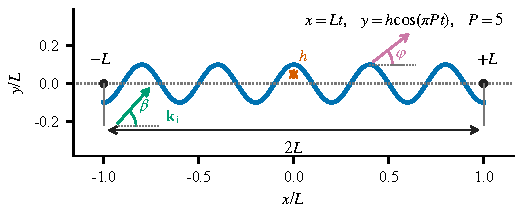
\includegraphics[width=\columnwidth]{fig1_geometry.pdf}
 \caption{Symmetric finite sinusoidal PEC grating and angle convention.  The
 incident propagation direction is
 $\widehat{\boldsymbol d}=(\cos\beta,\sin\beta)$; observation angle $\varphi$
 is measured counterclockwise from $+x$.}
 \label{fig:geometry}
\end{figure}

With the suppressed time factor $e^{-i\omega t}$, a unit-amplitude incident
plane wave is
\begin{equation}
 U^{\rm inc}(\boldsymbol r)
 =\exp\!\left(ik\widehat{\boldsymbol d}\mathbin{\cdot}\boldsymbol r\right),
 \qquad
 \widehat{\boldsymbol d}=(\cos\beta,\sin\beta).
 \label{eq:incident}
\end{equation}
Thus constant-phase fronts travel along $\widehat{\boldsymbol d}$.  The
reported computations use normal incidence, $\beta=\pi/2$, so the wave travels
from the lower to the upper halfspace; no such restriction is made in the
equations.  The scattered field $U^{\rm sc}$ satisfies the Helmholtz equation,
the outgoing Sommerfeld condition, local energy finiteness at both endpoints,
and
\begin{equation}
 U^{\rm inc}+U^{\rm sc}=0 \quad \text{on }\Gamma .
 \label{eq:pec}
\end{equation}
The outgoing Green kernel is consequently $H_0^{(1)}$.

\subsection{Edge-Conditioned Integral Equation}

Absorb the constant in the electromagnetic Green function into a scaled line
density $q$.  Its known endpoint behavior is factored as
\begin{equation}
 q(t)|\boldsymbol r'(t)|
 =\frac{v(t)}{\pi\sqrt{1-t^2}},
 \label{eq:edgefactor}
\end{equation}
where $v$ is smooth.  Equation~\eqref{eq:edgefactor} extracts the singular
factor; it does not remove the physical edge singularity.  The scattered field
and the logarithmically singular integral equation (IE) are then written using
$\rho_t=|\boldsymbol r-\boldsymbol r(t)|$ and
$R(t,\tau)=|\boldsymbol r(t)-\boldsymbol r(\tau)|$, with
$G(s)=H_0^{(1)}(ks)$, $w(t)=(1-t^2)^{-1/2}$, and
$u_0(\tau)=U^{\rm inc}(\boldsymbol r(\tau))$:
\begin{align}
 U^{\rm sc}(\boldsymbol r)
 &=\frac{1}{\pi}\int_{-1}^{1}
 G(\rho_t)
 v(t)w(t)\,dt,                                                       \label{eq:potential}\\
 \frac{1}{\pi}\int_{-1}^{1}
 G\!\left(R(t,\tau)\right)
 v(t)w(t)\,dt
 &=-u_0(\tau).                                                       \label{eq:ie}
\end{align}
The explicit $1/\pi$ makes the continuous and discrete normalizations
transparent.

First, the logarithmically singular IE~\eqref{eq:ie} is differentiated with
respect to $\tau$, giving a Cauchy-singular IE.  Second, that equation is
discretized.  In particular, let
\begin{align}
 c_H&=-\frac{2i}{\pi},                                                   \label{eq:ch}\\
 K(t,\tau)&=\frac{\partial}{\partial\tau}
 H_0^{(1)}\!\left(kR(t,\tau)\right)-\frac{c_H}{t-\tau},                 \label{eq:kernel}\\
 f(\tau)&=-\frac{d}{d\tau}U^{\rm inc}(\boldsymbol r(\tau))
 =-ikU^{\rm inc}(\boldsymbol r(\tau))
 \widehat{\boldsymbol d}\mathbin{\cdot}\boldsymbol r'(\tau).
 \label{eq:rhs}
\end{align}
The coefficient $c_H$ follows directly from the small-argument expansion of
$H_0^{(1)}$; with it, $K$ has a finite diagonal limit.  The differentiated
equation is
\begin{equation}
 \frac{1}{\pi}\operatorname{p.v.}\!\int_{-1}^{1}
 \left[\frac{c_H}{t-\tau}+K(t,\tau)\right]
 \frac{v(t)}{\sqrt{1-t^2}}\,dt=f(\tau).
 \label{eq:cauchyie}
\end{equation}

Use the Gauss--Chebyshev nodes and the interlaced second-kind points
\begin{align}
 t_i&=\cos\frac{(2i-1)\pi}{2N},&&i=1,\ldots,N, \notag\\
 \tau_j&=\cos\frac{j\pi}{N},&&j=1,\ldots,N-1.                    \label{eq:nodes}
\end{align}
Writing $v_i=v(t_i)$, the implementation returns these samples as
\texttt{v\_nodes}.  Thus its publication-facing density already includes the
factor $\pi$ relative to a convention that retains the quadrature weight
$\pi/N$.
For $j=1,\ldots,N-1$, the boundary rows are
\begin{equation}
 \frac{1}{N}\sum_{i=1}^{N}
 \left[\frac{c_H}{t_i-\tau_j}+K(t_i,\tau_j)\right]v_i=f(\tau_j).
 \label{eq:nystrom}
\end{equation}
The $1/N$ factor is precisely the Gauss--Chebyshev weight $\pi/N$ combined
with the $1/\pi$ in~\eqref{eq:cauchyie}.

Differentiation loses one constant.  Equivalence to~\eqref{eq:ie} is restored
with one supplementary row,
\begin{equation}
 \frac{1}{N}\sum_{i=1}^{N}M(t_i)v_i=c,                                  \label{eq:supprow}
\end{equation}
where
\begin{align}
 M(t)&=\int_{-1}^{1}H_0^{(1)}\!\left(kR(t,\tau)\right)
          \frac{d\tau}{\sqrt{1-\tau^2}},                                \label{eq:mdef}\\
 c&=-\int_{-1}^{1}U^{\rm inc}(\boldsymbol r(\tau))
          \frac{d\tau}{\sqrt{1-\tau^2}}.                               \label{eq:cdef}
\end{align}
The logarithmic self term in $M$ is subtracted analytically and its smooth
remainder is evaluated by a higher-order Chebyshev rule.  Equations
\eqref{eq:nystrom} and~\eqref{eq:supprow} form an $N\times N$ dense system.

\subsection{Far Field and TSCS}

For $\widehat{\boldsymbol s}(\varphi)=(\cos\varphi,\sin\varphi)$, define
$\Phi_{\rm sc}$ by
$U^{\rm sc}(r,\varphi)\sim e^{ikr}\Phi_{\rm sc}(\varphi)/\sqrt{kr}$.
The same quadrature gives
\begin{equation}
 \Phi_{\rm sc}^{(N)}(\varphi)
 =\sqrt{\frac{2}{\pi i}}\,\frac{1}{N}\sum_{i=1}^{N}
 e^{-ik\widehat{\boldsymbol s}(\varphi)\cdot\boldsymbol r(t_i)}v_i.
 \label{eq:farfield}
\end{equation}
For unit incident amplitude, the differential and total scattering
cross sections are
\begin{equation}
 \frac{d\sigma}{d\varphi}=\frac{|\Phi_{\rm sc}(\varphi)|^2}{k},
 \qquad
 \sigma=\frac{1}{k}\int_{0}^{2\pi}|\Phi_{\rm sc}(\varphi)|^2\,d\varphi.
 \label{eq:tscs}
\end{equation}
Both have the required length dimension.  The polar plots below display the
absolute quantity $10\log_{10}[(d\sigma/d\varphi)/L]$; they are not normalized
to the maximum of each curve.

For reference, the infinite periodic continuation has tangential harmonics
\begin{equation}
 \xi_m=\cos\beta+\frac{m\pi P}{kL},\qquad |\xi_m|<1.                    \label{eq:floquet}
\end{equation}
Their upper- and lower-halfspace angles are $\arccos\xi_m$ and
$2\pi-\arccos\xi_m$, respectively.  These angles are only markers for the
broad lobes of the finite grating; below they are called infinite-grating
reference directions.  At normal incidence this reduces to
\begin{equation}
 \cos\varphi_m=\frac{m\pi P}{kL},\qquad
 \left|\frac{m\pi P}{kL}\right|<1.                                    \label{eq:floquetnormal}
\end{equation}
The first-order
markers become propagating at
\begin{equation}
 kL=\pi P=\FirstOrderCutoff \quad (P=5).                                 \label{eq:cutoff}
\end{equation}

\begin{figure*}[!t]
 \centering
 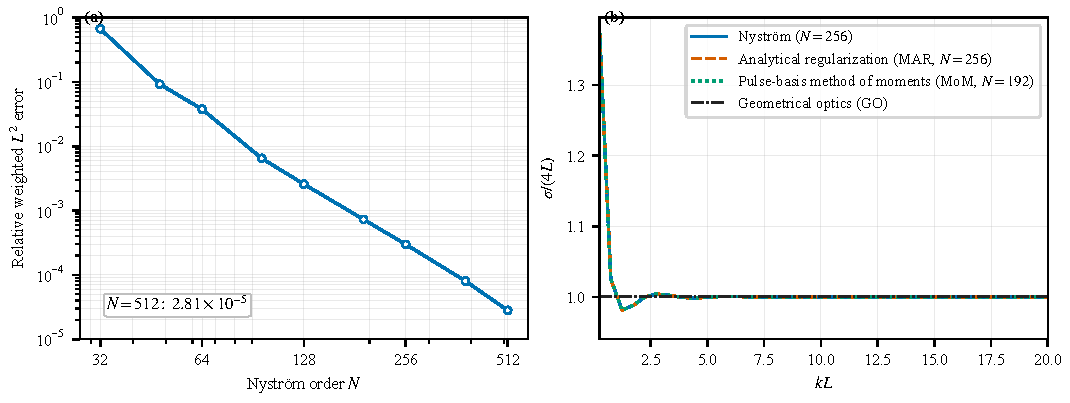
\includegraphics[width=\textwidth]{fig2_verification.pdf}
 \caption{Verification. (a) Relative $L^2$ error of the smooth density versus
 interpolation order for $P=5$, $h/L=0.10$, and $kL=20$.
 (b) Flat-strip total scattering cross section (TSCS), normalized by its
 geometrical-optics limit $4L$, from the differentiated Nystr\"om method
 ($N=256$), the method of analytical regularization (MAR; $N=256$), and a
 pulse-basis method of moments (MoM; 192 elements); the dash-dotted line is the
 geometrical-optics (GO) limit.}
 \label{fig:verification}
\end{figure*}

\section{Numerical Results}
\label{sec:results}

\subsection{Convergence and Cross-Validation}

Fig.~\ref{fig:verification}(a) reports a relative weighted $L^2$ error of
the smooth density for $P=5$, $h/L=0.10$, $kL=20$, and $\beta=\pi/2$.  Let
$I_Nv_N$ denote its Chebyshev interpolant and set
$\theta_\ell=(\ell+1/2)\pi/4096$.  With the $N_{\rm ref}=800$ solution as the
reference, the plotted error is
\begin{equation}
 \epsilon_N=\left[
 \frac{\sum_{\ell=0}^{4095}|I_Nv_N(\cos\theta_\ell)
       -I_{800}v_{800}(\cos\theta_\ell)|^2}
      {\sum_{\ell=0}^{4095}|I_{800}v_{800}(\cos\theta_\ell)|^2}
 \right]^{1/2}.
 \label{eq:l2error}
\end{equation}
This midpoint sampling in $\theta$ approximates the
$L^2_{1/\sqrt{1-t^2}}$ norm in $t$.  For
$N=32,48,64,96,128,192,256,384,512$, the error decreases systematically and
reaches \ConvErrorNFiveTwelve at $N=512$.  The latter order is used for all
corrugated-grating results below.  Repeating every unique publication case at
$N=800$ changes the TSCS by at most \ProductionMaxTSCSChange and the full
complex far-field pattern by at most \ProductionMaxPatternChange in relative
$L^2$ norm.

The second test uses a flat strip ($h=0$) over 41 electrical sizes
$0.25\leq kL\leq20$.  Fig.~\ref{fig:verification}(b) compares the present
differentiated Nystr\"om implementation with separately assembled
analytical-regularization and pulse-basis method-of-moments backends.  The
maximum spread in $\sigma/(4L)$ among the three results is \BackendMaxDiff.
The first two use $N=256$, and the pulse discretization uses 192 elements.
At the most demanding endpoint, $kL=20$, doubling those orders changes the
TSCS by at most \FlatOrderDoublingMaxChange.
At $kL=20$ the Nystr\"om value is
\FlatTSCSRatioTwenty.  This is close to the geometrical-optics limit
$\sigma/(4L)\to1$ for a broadside-illuminated flat PEC strip of projected
width $2L$~\cite{shapoval2011}, but it is correctly retained as a
finite-frequency value.

\subsection{Representative Five-Period Grating}

Fig.~\ref{fig:fieldpattern} shows the normal-incidence solution for
$P=5$, $h/L=0.10$, and $kL=20$.  The total-field intensity is shown relative
to the unit incident-field intensity.  Below the grating, incident and reflected fields
interfere; above it, the pattern contains the shadow lobe.  The
polar panel gives the absolute differential cross section over $0\leq
\varphi<2\pi$.  At this electrical size the $m=\pm1$ periodic-reference
harmonics are propagating, and the calculated finite-grating pattern contains
broad off-normal structure near their infinite-grating reference directions.
The central
reflection lobe and end-generated background remain present because only five
periods are retained.

\begin{figure*}[!t]
 \centering
 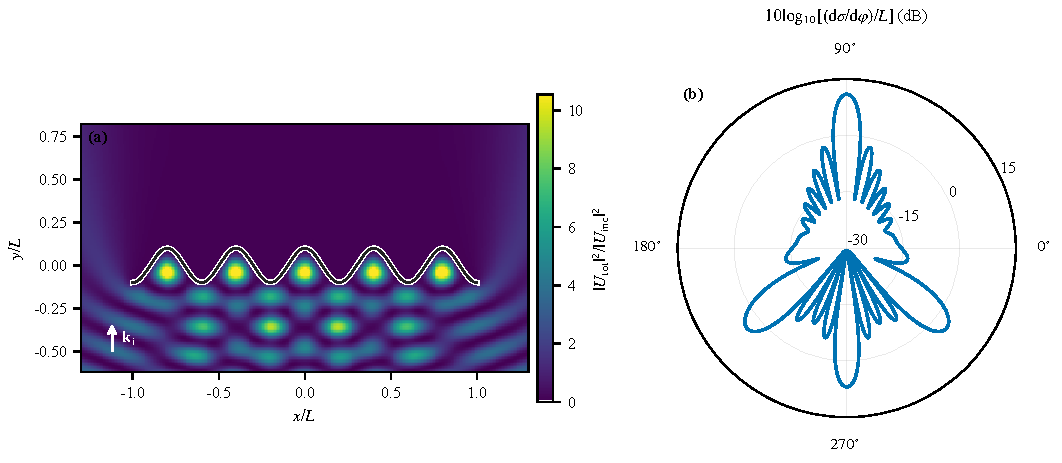
\includegraphics[width=0.83\textwidth]{fig3_field_pattern.pdf}
 \caption{Five-period grating at $P=5$, $h/L=0.10$, $kL=20$, and
 $\beta=\pi/2$. (a) Relative total-field intensity
 $|U^{\rm inc}+U^{\rm sc}|^2/|U^{\rm inc}|^2$. (b) Absolute polar
 differential scattering cross section, shown as
 $10\log_{10}[(d\sigma/d\varphi)/L]$ on the common $-30$ to $+15$ dB scale.}
 \label{fig:fieldpattern}
\end{figure*}

\subsection{Height and Electrical-Size Dependence}

At fixed $P=5$ and $kL=20$, increasing $h/L$ changes the phase and magnitude
of the induced current across each corrugation.  Fig.~\ref{fig:amplitude}
shows the resulting redistribution among the specular and off-normal lobes.
Because every panel has the same absolute radial scale, changes in level can be
compared directly.  The normalized TSCS values for $h/L=0$, $0.05$, and
$0.10$ are, respectively,
\begin{equation}
 \frac{\sigma}{4L}=
 \AmpTSCSFlat,\quad \AmpTSCSFive,\quad \AmpTSCSTen.
 \label{eq:ampvalues}
\end{equation}
Thus corrugation changes both the angular distribution and the integrated
scattered power; the polar curves are not merely rescaled copies.

\begin{figure*}[!t]
 \centering
 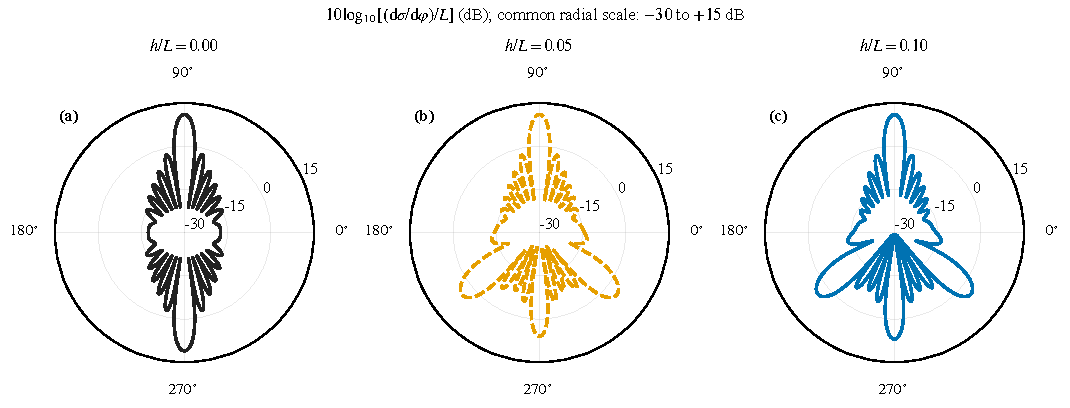
\includegraphics[width=0.83\textwidth]{fig4_amplitude_polar.pdf}
 \caption{Absolute polar differential scattering cross section, shown as
 $10\log_{10}[(d\sigma/d\varphi)/L]$, for $P=5$, $kL=20$, and
 $\beta=\pi/2$: (a) $h/L=0$; (b) $h/L=0.05$; and (c) $h/L=0.10$. Each
 panel contains one curve and uses the common $-30$ to $+15$ dB scale.}
 \label{fig:amplitude}
\end{figure*}

Frequency changes both the overall electrical width and the set of
propagating periodic-reference harmonics.  For $P=5$ and $h/L=0.10$, the
three cases in Fig.~\ref{fig:frequency} have
\begin{align}
 \frac{\sigma}{4L}&=\FreqTSCSTwelve,&&kL=12, \notag\\
 &=\FreqTSCSSixteen,&&kL=16, \notag\\
 &=\FreqTSCSTwenty,&&kL=20.                              \label{eq:freqvalues}
\end{align}
\begin{figure*}[!t]
 \centering
 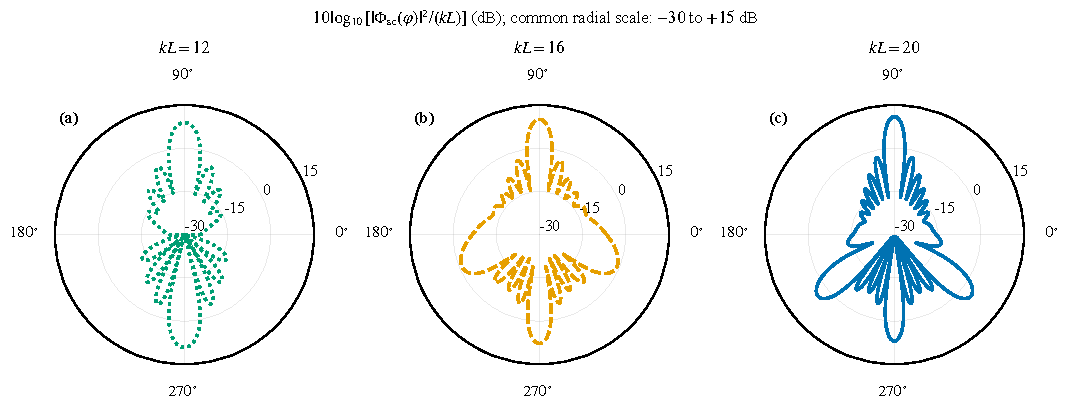
\includegraphics[width=0.83\textwidth]{fig5_frequency_polar.pdf}
 \caption{Absolute polar differential scattering cross section, shown as
 $10\log_{10}[(d\sigma/d\varphi)/L]$, for $P=5$, $h/L=0.10$, and
 $\beta=\pi/2$: (a) $kL=12$; (b) $kL=16$; and (c) $kL=20$. Each panel
 contains one curve and uses the common $-30$ to $+15$ dB scale. The
 first-order periodic-reference harmonics are cut off at $kL=5\pi$ and
 propagate above it.}
 \label{fig:frequency}
\end{figure*}

At $kL=12$ the first-order periodic harmonics are evanescent.  They become
propagating above the threshold in~\eqref{eq:cutoff}, so first-order
finite-grating lobes appear in the $kL=16$ pattern and separate further from
their cutoff directions at $kL=20$.  Their finite width and interaction with
the background preclude interpreting them as exact diffraction orders.

\section{Conclusion}

An edge-conditioned integral equation, discretized with the Nystr\"om
technique, has been formulated for E-polarized plane-wave scattering by a
finite sinusoidal PEC grating.  The formulation accommodates arbitrary
incidence, uses the outgoing $H_0^{(1)}$ kernel consistently with
$e^{-i\omega t}$, and retains the correct $1/k$ factor in the TSCS.  Density
convergence, agreement among three separately implemented formulations, and the approach of
the flat-strip result to its geometrical-optics limit provide complementary
accuracy checks.  For the five-period grating, height mainly redistributes
scattering among angular lobes, whereas electrical size determines when
periodic-reference harmonics become propagating.  Absolute polar plots and
the reported $\sigma/(4L)$ values show that both redistribution and total
scattered power vary with the profile.

\IEEEtriggeratref{2}
\begin{thebibliography}{00}

\bibitem{nazarchuk1989}
Z.~T. Nazarchuk, \emph{Numerical Investigation of Wave Diffraction from
Cylindrical Structures}. Kyiv, Ukraine: Naukova Dumka, 1989, in Russian.

\bibitem{shapoval2011}
O.~V. Shapoval, R. Sauleau, and A.~I. Nosich, ``Scattering and absorption of
waves by flat material strips analyzed using generalized boundary conditions
and Nystr\"om-type algorithm,'' \emph{IEEE Trans. Antennas Propag.}, vol. 59,
no. 9, pp. 3339--3346, Sep. 2011, doi: 10.1109/TAP.2011.2161547.

\bibitem{kobayashi1991}
K. Kobayashi and T. Eizawa, ``Plane wave diffraction by a finite sinusoidal
grating,'' \emph{IEICE Trans. Electron.}, vol. E74-C, no. 9, pp. 2815--2826,
Sep. 1991, doi: 10.1587/e74-c\_9\_2815.

\bibitem{eizawa2014}
T. Eizawa and K. Kobayashi, ``Wiener--Hopf analysis of the H-polarized plane
wave diffraction by a finite sinusoidal grating,'' \emph{Prog.
Electromagn. Res.}, vol. 149, pp. 1--13, 2014,
doi: 10.2528/PIER14063007.

\bibitem{vinogradova2019}
E.~D. Vinogradova, K. Kobayashi, and T. Eizawa, ``Full wave analysis of plane
wave diffraction by a finite sinusoidal grating: E-polarization case,''
\emph{Wave Motion}, vol. 86, pp. 44--62, Mar. 2019,
doi: 10.1016/j.wavemoti.2018.12.006.

\bibitem{vinogradova2021}
E.~D. Vinogradova and K. Kobayashi, ``Complex eigenvalues of natural
TM-oscillations in an open resonator formed by two sinusoidally corrugated
metallic strips,'' \emph{IET Microw., Antennas Propag.}, vol. 15, no. 10,
pp. 1283--1298, 2021, doi: 10.1049/mia2.12166.

\end{thebibliography}

\end{document}
